\chapter{Background}
    \section{Evolution of Digital Signal Processors}
        A digital signal processor (DSP) is an optimized computer that aims at accelerating digital signal processing, such as baseband demodulation or video codec.
        In principle, a programmer extracts key subroutines or algorithms from applications and accelerates them with a DSP.
        Such extracted pieces of code executed by DSPs are also referred to DSP kernels.
        Unlike a general purpose computers, which usually feature powerful ISA and novel branch predictors that help them with control intensive tasks,
        DSPs simply focus on computation intensive tasks delivered by another unit (general purpose processor, analog to digital converter, etc.), 
        and thus its hardware can be simplified and optimized for better power efficiency, which enable them to be widely used in mobile devices and embedded systems.
        \\\indent
        The single-issue reduced instruction set computer (scalar), introduced in 1980s \cite{risc}, has become a popular template for DSP owing to its simplicity.
        The key concept of scalar is designing an ISA with primitive and orthogonal instructions which demand simpler datapath.
        By taking the advantage of the regularity in its datapath, pipelining technique can thus be adopt to achieve the application requirement.
        However, two drawbacks still exist in scalar. 
        The first its lack of instruction-level parallelism (ILP). 
        Functional units are not able to work concurrently due to the limitation of the single-issue datapath.
        This can be resolved by designing a multi-issue datapath with either hardware (i.e., superscalar) or software (i.e., VLIW) instruction scheduling.
        In the field of DSP design, adopting the VLIW architecture is a preferable strategy, 
        because hardware simplicity matters than portability and many optimization approaches can be applied in compilation stages. 
        Fig.~\ref{fig:vliw} illustrates a 3-way issue VLIW datapath, where three instructions can be dispatched at a cycle.
        The number of ports on RF is scaled up with the issue-width, and the compiler is responsible for performing static scheduling to avoid resources conflict among operations.
        \vspace{\textfig}
        \begin{figure}[!ht] 
            \centering
            \includegraphics[width=0.5\textwidth]{./figs/vliw.eps}
            \caption{Basic VLIW datapah}
            \label{fig:vliw}
        \end{figure}
        \\\indent
        The second drawback of scalar is plenty of redundant writing back (WB) to RF. 
        In digital signal processing, intermediate results are often read exactly once, which implies lots of RF storage of them is redundant.
        Several approaches have been proposed to address this issue.
        Fig.~\ref{fig:cascade} shows the datapath of the composite-ALU architecture that cascades primitive arithmetic units. 
        Intermediate results can be forwarded from one to its follower with an optimized order which targets specific applications.
        The processor with such customization in the datapath is referred to as application-specific instruction set processor (ASIP).
        \vspace{\textfig}
        \begin{figure}[!ht] 
            \centering
            \includegraphics[width=0.6\textwidth]{./figs/cascade.eps}
            \caption{Composite-ALU architecture}
            \label{fig:cascade}
        \end{figure}
        \\\indent
        Another approach that enables forwarding mechanism even further is shown in Fig.~\ref{fig:tta}, where FUs, RF and load/store units are linked by an interconnection network (ICN).
        Such an architecture makes a significant distinction from scalar because only a "move" instruction is needed. 
        All computation can be completed by moving operands on the interconnection network, avoiding WB as much as possible.
        \vspace{\textfig}
        \begin{figure}[!ht] 
            \centering
            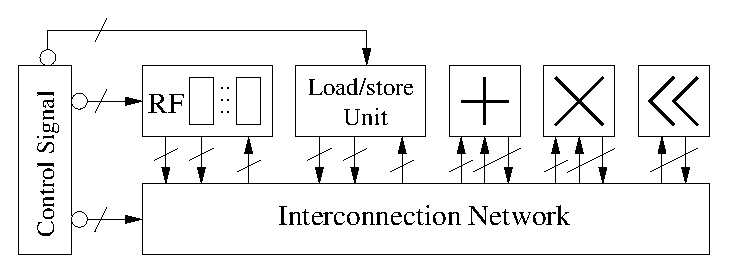
\includegraphics[width=0.8\textwidth]{./figs/tta.eps}
            \caption{Transport triggered architecture (TTA)}
            \label{fig:tta}
        \end{figure}
      
        %\subsection{Application-Specific Instruction Set Processor}
        %\subsection{Very Long Instruction Word Processor}
        %\subsection{Transport-Triggered Architecture}

    %\section{Register File Model}
    %Register file (RF) organization also serves as an important role in DSP design. 
    %Increaing computational demand drives more and more FUs on RF,
    %which result in significant hardware cost.
    %In this part, we will introduce a basic RF model to explain hardware cost in area, delay and power perspectives.
    %\subsection{Area}
    %\label{sec:area}
    %RF is an array of register cells, each of which connects to several bit lines and word lines.
    %Fig.~\ref{fig:rf} illustrates a basic schematic of a register cell.
    %    \vspace{\textfig}
    %    \begin{figure}[!ht] 
    %        \centering
    %        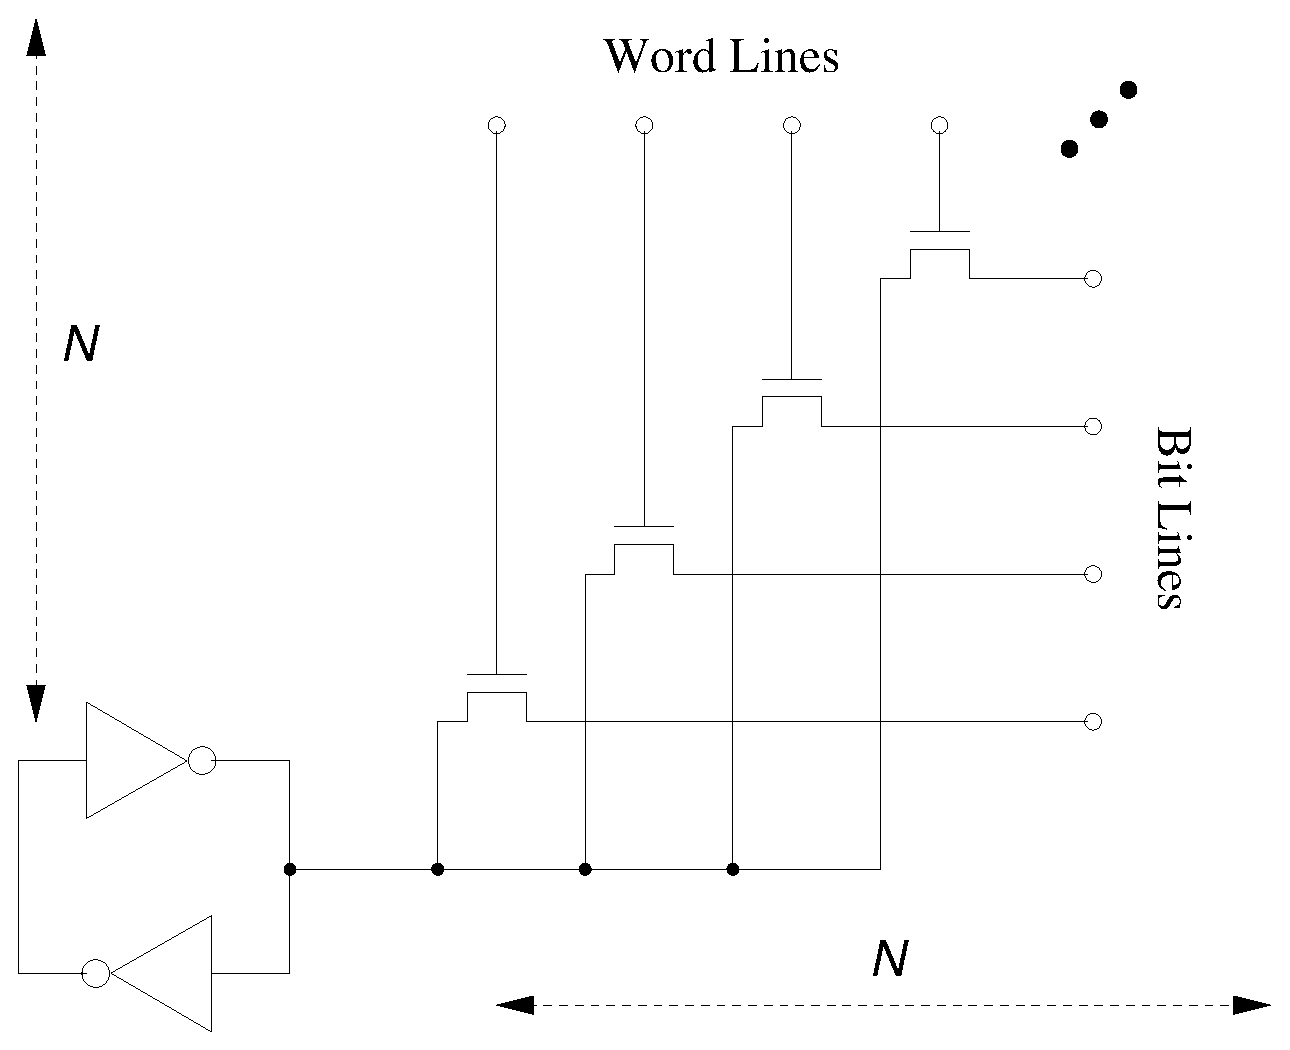
\includegraphics[width=0.7\textwidth]{./figs/rf.eps}
    %        \caption{Register cell schematic}
    %        \label{fig:rf}
    %    \end{figure}
    %For a centralized RF organization with N ports, 
    %each register cell is connected to N bit lines, each of which controlled by a word lines.
    %N bit lines and N word lines are placed horizontally and vertically respectively.
    %Since the width of wire tracks is a constant, 
    %the interconnection area of each cell grows with the factor of $N^2$.
    %Moreover, since the register number grows with the FU number as well,
    %the factor of total interconnection area is further multiplied with another N and reaches $N^3$,  
    %which dominates the chip area when N is large.
    %\subsection{Delay}
    %Wire propagation and fan-out/fan-in delays are two major constituents of RF access delay.
    %The former is the latency of a logic passage across a wire,
    %which is proportional to the wire length, 
    %while the latter is the latency of driving on capacitive loads.
    %As discussed in ~\ref{sec:area}, the interconnection area of RF is the factor of $N^3$.
    %By taking square root on the factor of area, 
    %we obtain another factor, $N^{3/2}$, for wire length and propagation delay.
    %The growing wire length increases load capacitance on bit lines as well, 
    %and it contribute additional fan-out/fan-in delay to the overall.
    %Nevertheless, $N^{3/2}$ is still the dominating factor of RF access delay when N is large.
    %\subsection{Power}
    %For each access to RF, bit lines need to be pre-charged to a threshold voltage,
    %and then sense register cells by asserting specific word lines.
    %As a result, the energy dissipation in RF is mainly resulted from logic switching in bit lines capacitance,
    %because every bit line dedicated to a port needs to be active to accomplish an access to the port.
    %As the port number increases, the capacitance in bit line is principally wire capacitance.
    %The overall power consumption of bit lines grows with the product of the bit line number and the wire length.
    %As shown in Fig.~\ref{fig:rf}, the wire length and the bit line number of each cell are proportional to N.
    %Since the register cell number is proportional to N as well, 
    %the overall power consumption of bit lines is also the factor of $N^3$ when N is large.
    %    %\subsection{Centralized Register Files}
        %\subsection{Banked Register Files}
        %\subsection{Clustered Register Files}
        %\subsection{Distributed Register Files}
    \section{Heterogeneous System Architecture}
    \textit{Heterogeneous System Architecture} (HSA) presents an unified view of various computing devices, 
    such as CPU, DSP, GPU and FPGA.
    HSA allows these devices to be integrated in a single system heterogeneously, and even share the same memory virtually or physically.
    Such asymmetry of computing devices in HSA is the key differentiation from conventional symmetric multiprocessing (SMP) \cite{parallel},
    which involves two or more identical processors collaborating with uniform access to the shared memory.
    By adopting HSA, one is able to design a single system that handles wide variety of computational demands efficiently.
    For example, in 2014, AMD released its fourth generation of the Accelerated Processing Unit (APU), \textit{Carrizo APU} \cite{carrizo}, featuring HSA 1.0.
    As illustrated in Fig.~\ref{fig:carrizo}, \textit{Carrizo} is the SoC platform with the 4-core CPU and the GPU with 8 compute units (384 shader cores totally).
    Both of them work with \textit{the Shared Virtual Memory} (SVM) since their MMUs access an identical page table.
    \textit{Carrizo} enables task sharing without data copy between CPUs and GPUs to achieve greater performance.
    By cleverly choosing the suitable computing device for each task, 
    \textit{Carrizo} can operate more efficiently to save power as well.
    Since the proposed DeAr DSP targets HSA platforms, 
    in this part, we will briefly introduce key features of HSA in three perspectives: 
    system specification, programming model and software infrastructure.
        \vspace{\textfig}
        \begin{figure}[!ht] 
            \centering
            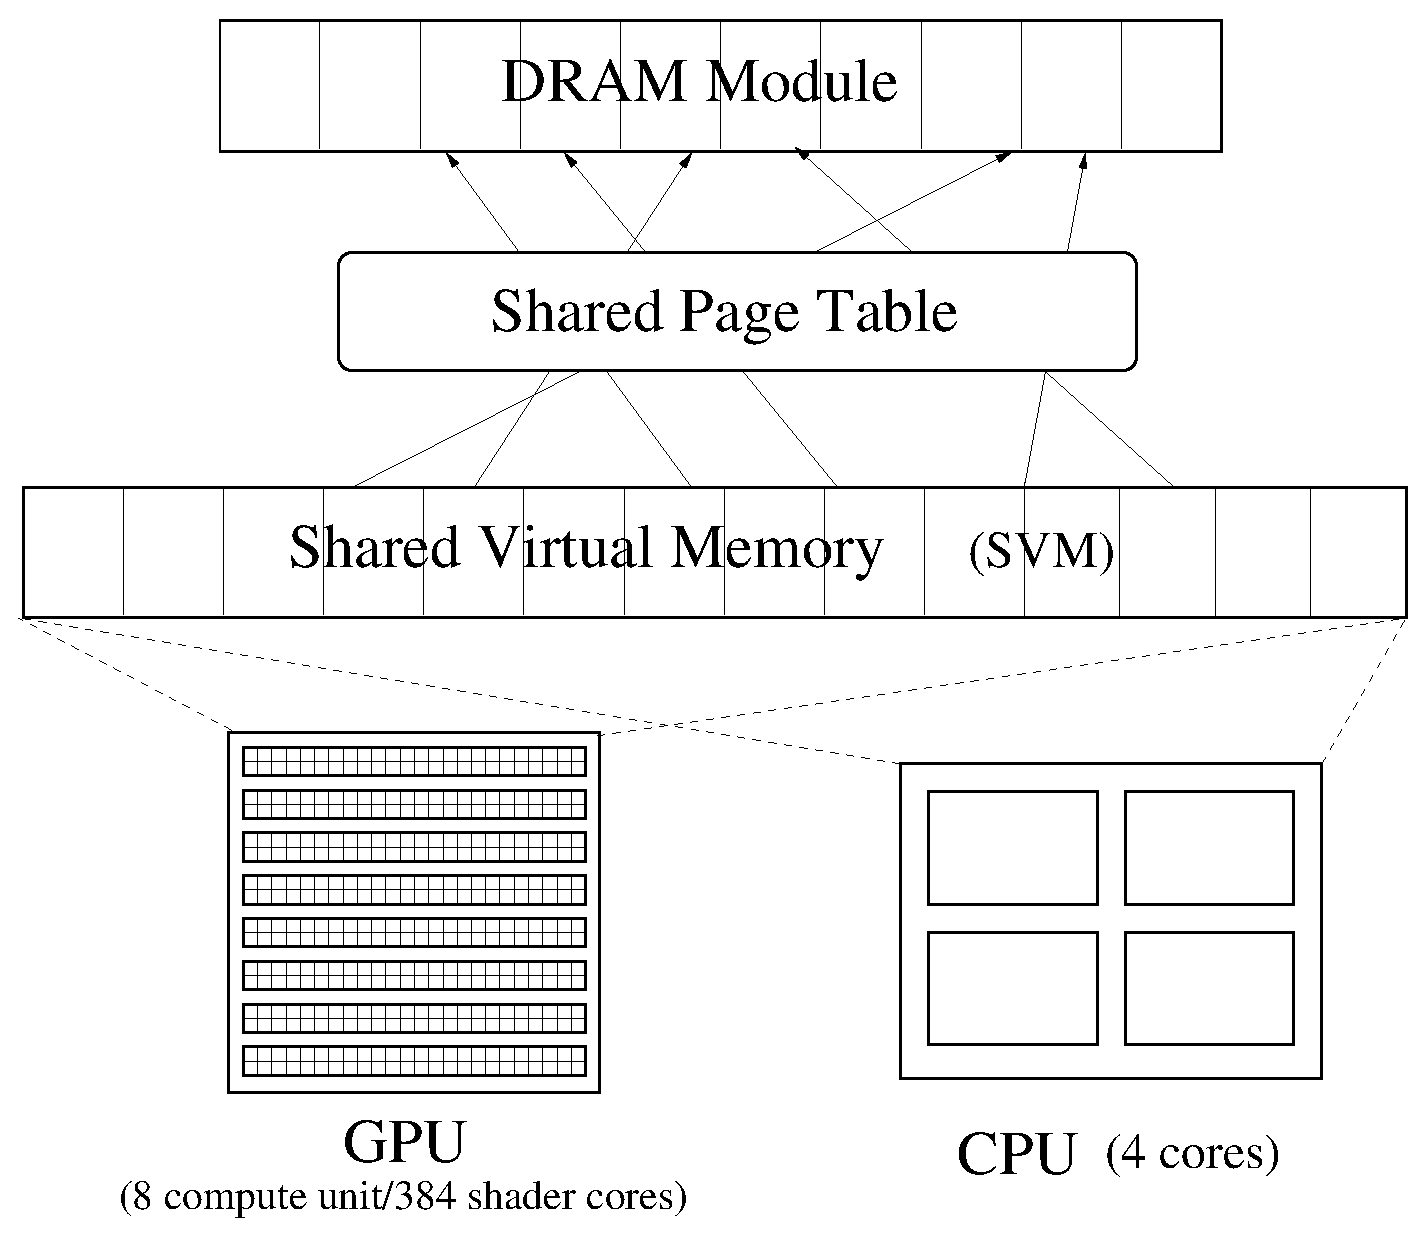
\includegraphics[width=0.8\textwidth]{./figs/carrizo.eps}
            \caption{Carrizo APU with HSA}
            \label{fig:carrizo}
        \end{figure}
        \subsection{System Specification}
        The HSA foundation released HSA Platform System Architecture Specification 1.0 \cite{systemspec} in 2015.
        The main purpose of the specification is defining the system requirements which support the HSA programming model and the software infrastructure, from a hardware perspective.
        Fig.~\ref{fig:systemspec} illustrates an example of an HSA platform.
        An HSA platform refers to a system involving multiple types of computing devices, 
        which are defined as HSA agents.
        One of the agents needs to be host CPU, and the other usually serve as kernel agents. 
        The host CPU is responsible for running the operating system and setting up \textit{HSA Runtime},
        while kernel agents handle computational tasks from the host CPU.
        HSA requires all HSA agents to be capable of accessing SVM maintained coherently, 
        so data exchange between agents can be accomplished by passing data pointer instead.
        Nevertheless, not all memory regions need to be accessible by all agents (i.e., \textit{Global} segment).
        HSA defines other memory segments (\textit{Group}, \textit{Private}, \textit{Spilled}, etc.), 
        which possess various accessibility by various computing agents or items.
        By manipulating different memory segments, the programmer can utilize data locality in memory hierarchy to improve performance.
        To transmit control signals between agents, HSA specifies \textit{Architected Queuing Language} (AQL) as the protocol. 
        AQL defines several packet types: \textit{agent dispatch}, \textit{kernel dispatch}, \textit{AND barrier} and \textit{OR barrier}, etc.
        An agent pushes tasks wrapped in \textit{kernel dispatch} or \textit{agent dispatch} packets to command queues, 
        and other agents consume the packets, and dispatch the wrapped tasks.
        \textit{AND barrier} and \textit{OR barrier} are pushed to command queues to synchronize execution of agents.
        Another advantage of AQL is allowing \textit{user mode queuing},
        which implies the programmer is allowed to access the command queue via \textit{HSA Runtime API} without OS involving.
        By this means, the latency from dispatching to execution of a task is thus minimized.
        \vspace{\textfig}
        \begin{figure}[!ht] 
            \centering
            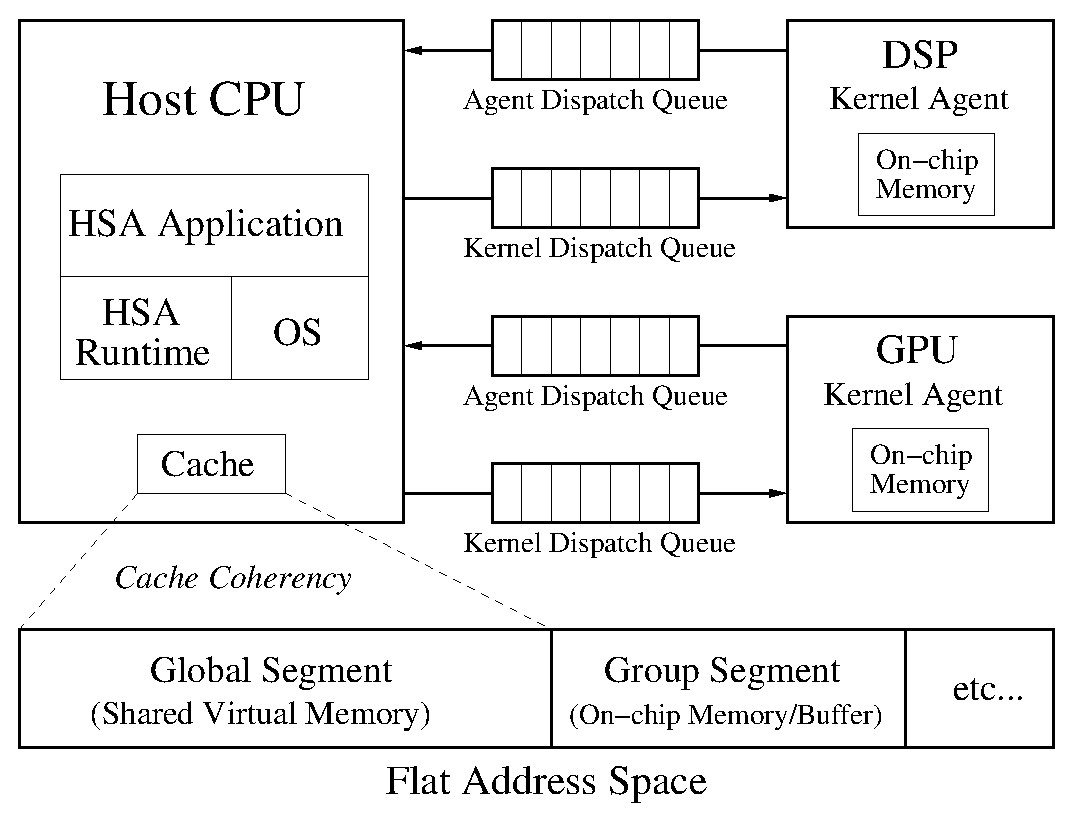
\includegraphics[width=0.85\textwidth]{./figs/systemspec.eps}
            \caption{Example of an HSA Platform}
            \label{fig:systemspec}
        \end{figure}
        \subsection{Programming Model}
        To support multiple Instruction Set Architectures (ISAs) for various agents in a single HSA platform,
        HSA foundation drew up \textit{Heterogeneous System Architecture Intermediate Language} (HSAIL)
        With HSAIL, programmers can develop code for HSA in an intermediate form accepted by wide range of agents.
        HSAIL basically adopts the parallel programming model of Single Program Multiple Data (SPMD), 
        which carries out same computation on different data to accelerate applications.
        HSAIL organizes instances of execution in specified hierarchy, which help programmers to manipulate its SPMD model.
        Fig.~\ref{fig:grid} presents a graphical view on how HSAIL organizes instances of execution.
        The atomic instance for execution is a work-item, which has dedicated registers and private memory.
        Group of work-items form a work-group, which owns group memory accessed by subordinate work-items only.
        The work-items in a work-group can be arranged in one, two or three dimensional coordinate, 
        and the programmer specifies the number of dimensions as well as the size of each dimension.
        Based on the same principle of arranging instances, all work-groups further form a grid, 
        which provides a global view to all work-items created in an HSAIL program (kernel).
        Work-items within a work-group are executed concurrently in chunks called wavefronts, 
        of which sizes are limited by the number of processing cores (lanes) in the target kernel agent.
        Each work-group and each work-item have work-group ID and work-item ID respectively.
        By manipulating such threading hierarchy, 
        the programmer can control accessibility of data and synchronize the work items in a specific scope without burden.
        \vspace{\textfig}
        \begin{figure}[!ht] 
            \centering
            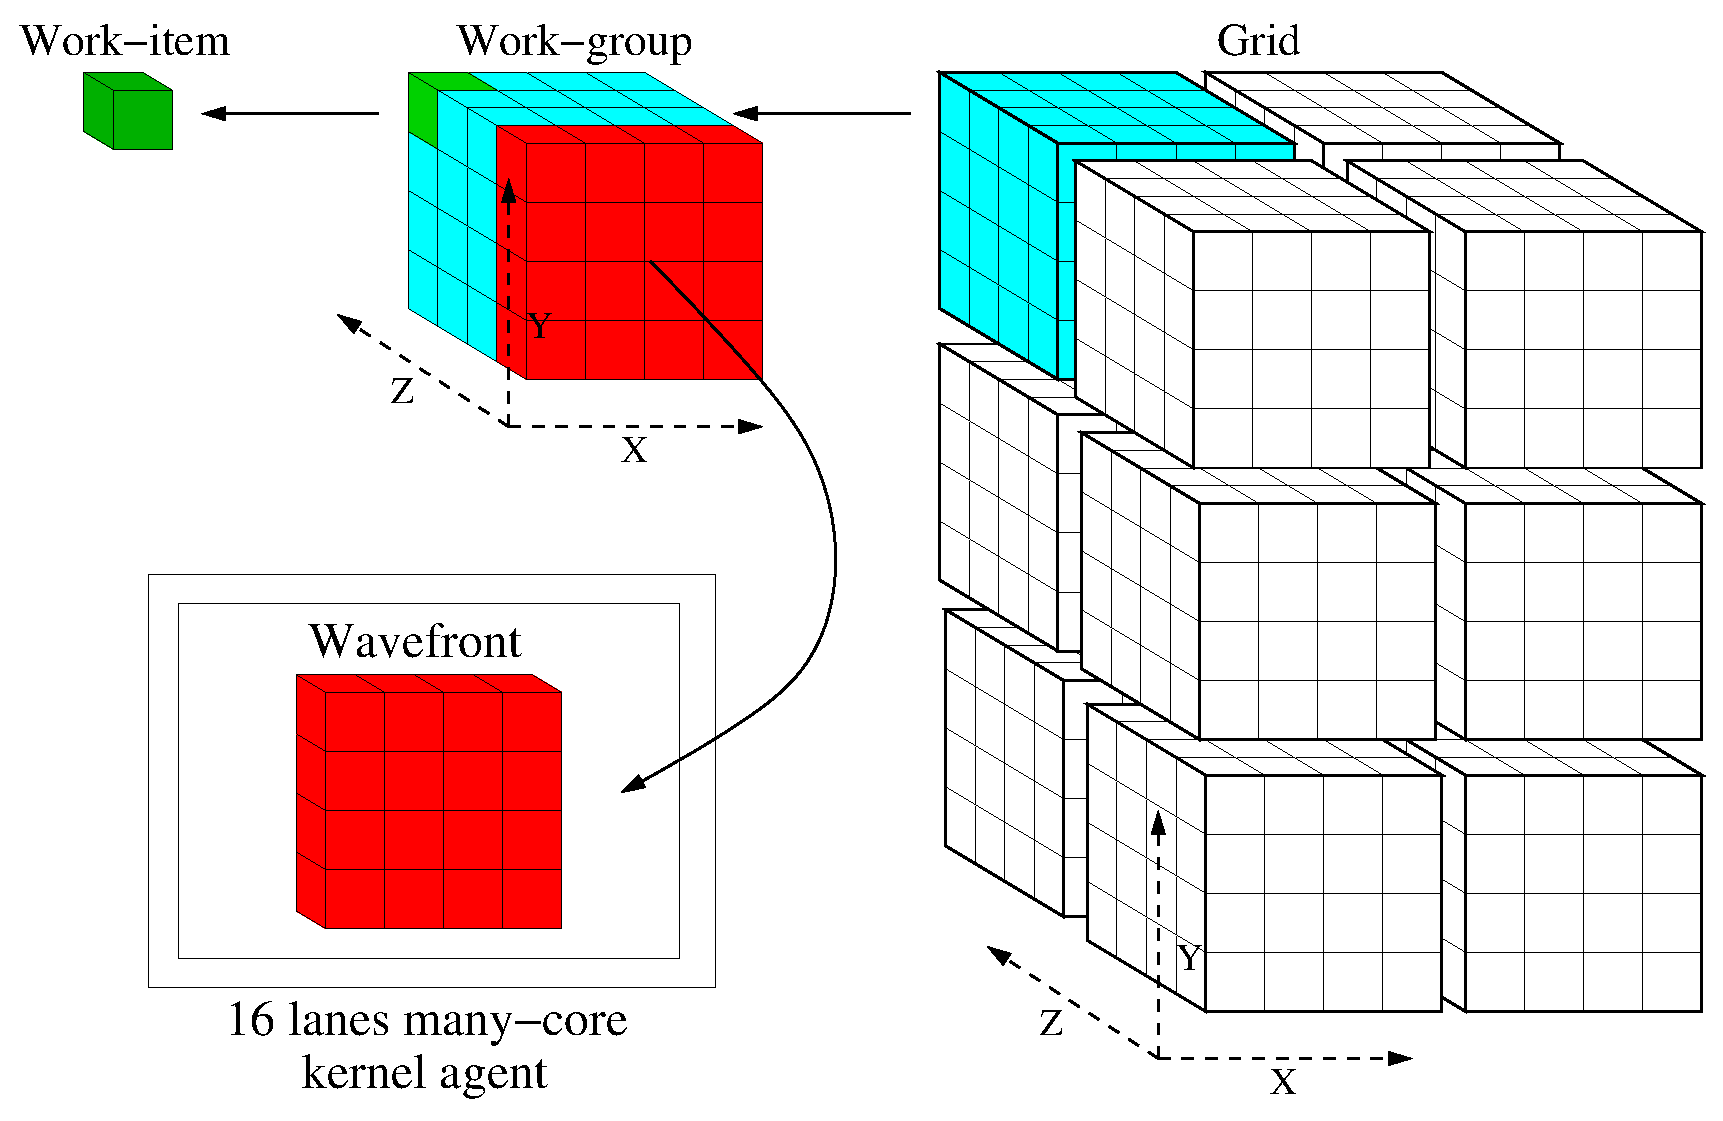
\includegraphics[width=0.85\textwidth]{./figs/grid.eps}
            \caption{Execution hierarchy in HSAIL}
            \label{fig:grid}
        \end{figure}
        % work group, work item warp, memory hierarchy, hqueue, 
        \subsection{Software Infrastructure}
        The software infrastructure of HSA is composed of two parts, the compilation tools and the \textit{HSA runtime}.   
        The compilation tools are responsible for generating machine code of specific ISAs from high-level language.
        Fig.~\ref{fig:swinf}~(a) illustrates the whole compilation flow of HSA software.
        The programmer develops applications targeting HSA with high-level parallel programming language such as OpenCL, OpenMP or a domain-specific language (DSL).
        The off-line compiler of the hight-level language translate the code to standard HSAIL kernel accepted by all computing devices in an HSA platform.
        Each kind of the computing devices must be recognized by the finalizer, 
        which is composed of several device-specific HSAIL compilers.
        Depending on which device is going to execute the kernel, 
        the finalizer translates the HSAIL to corresponding ISA and completes the code generation flow.
        \\\indent
        On the other hand, the \textit{HSA runtime} bridges HSA runtime APIs and agents, as illustrated in Fig.~\ref{fig:swinf}~(b).
        With the \textit{HSA runtime}, the programmer is allowed to manipulate system memory and AQL, 
        and thus SVM and \textit{user mode queuing} can be accomplished.
        It is possible that the programmer triggers the finalizer to perform the final stage of compilation at runtime.
        In addition, \textit{HSA runtime} also performs error handling and retrieve system and agent information for users.
        \vspace{\textfig}
        \begin{figure}[!ht] 
            \centering
            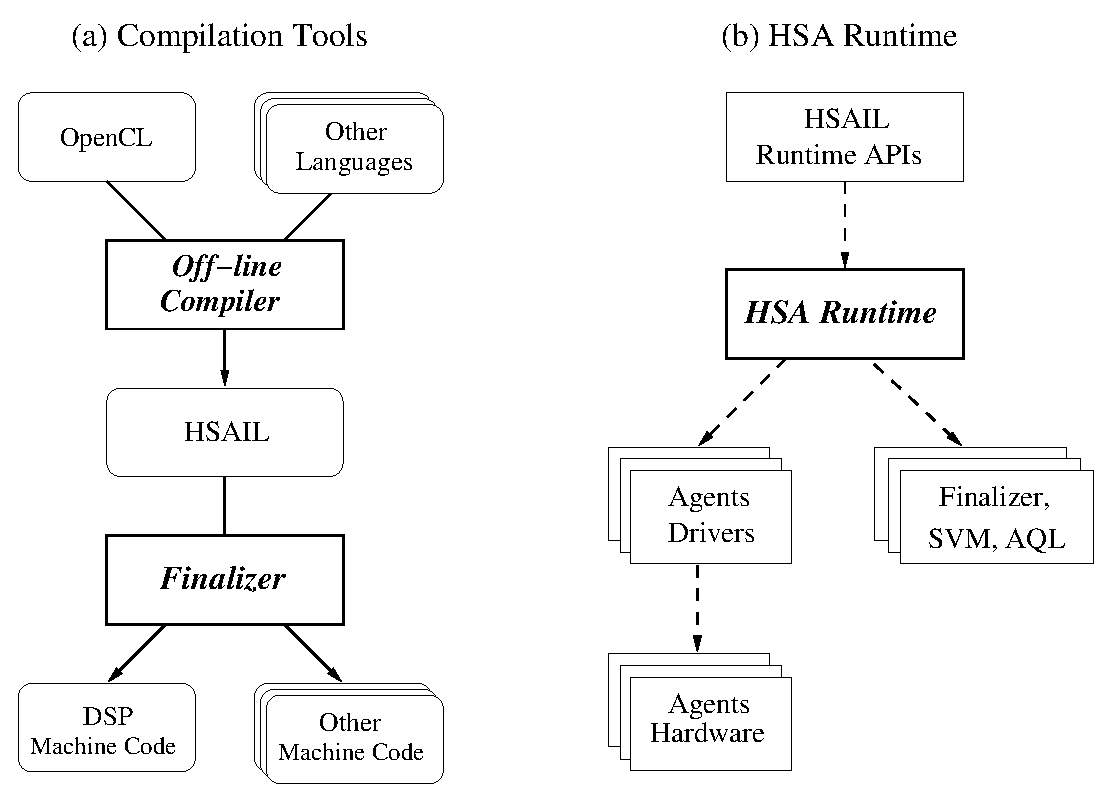
\includegraphics[width=0.85\textwidth]{./figs/swinf.eps}
            \caption{Software Infrastructe of HSA}
            \label{fig:swinf}
        \end{figure}

